\section{Wiremap}
The
Wiremap
is
an
innovative
projection
technique
that
builds
a
real
and
interactive
3d
image
by
manipulating
light
from
a
projector.

The
projector
throws
its
beam
on
an
array
of
vertical
wires
(the
number
of
wires
depends
on
your
desired
resolution).
From
the
focal
point
of
the
projector’s
lense,
all
the
wires
are
evenly
spaced
from
one
another.
However,
due
to
the
randomized
dimension
of
depth,
from
any
other
perspective,
the
wires
create
a
3‐D
map
of
cyberspace.
The
result
is
a
projection
screen
that
allows
for
the
visualization
of
a
2‐D
image
into
a
3‐D
object
whose
source
is
the
light
 of
a
projector.
An
object
can
move
around
and
change
in
color
or
size
according
to
whatever
is
delegated
by
the
programmer
in
Processing.




Our
specific
map
was
made
using
mason’s
string,
3⁄4
inch
plywood
and
some hardware
for
the
weighting
down
each
string
and
for
hanging
the
entire
wiremap
in space.
Our
map
used
256
strings
that
are
placed
in
a
randomized
dimension
of
depth through
256
holes
on
both
upper
and
lower
alignment
boards.
These
strings
are
secured
through
the
alignment
boards
at
the
top
and
bottom
with
hardware,
with
the
bottom
hardware
also
providing
an
element
of
weight
to
each
individual
string
to
keep
it
taught.
A
calibration
stage
must
be
done
after
initial
setup
of
the
wiremap,
this
process
aligns
the
top
and
bottom
boards
so
that
they
are
parallel
with
one
another.
Also,
the
focal
point
of
the
projector
must
be
properly
placed
in
line
with
the
wiremap
so
that
each
of
the
256
strings
contains
only
one
pixel
width
on
its
projection
surface.


\begin{figure}[htp]\centering
  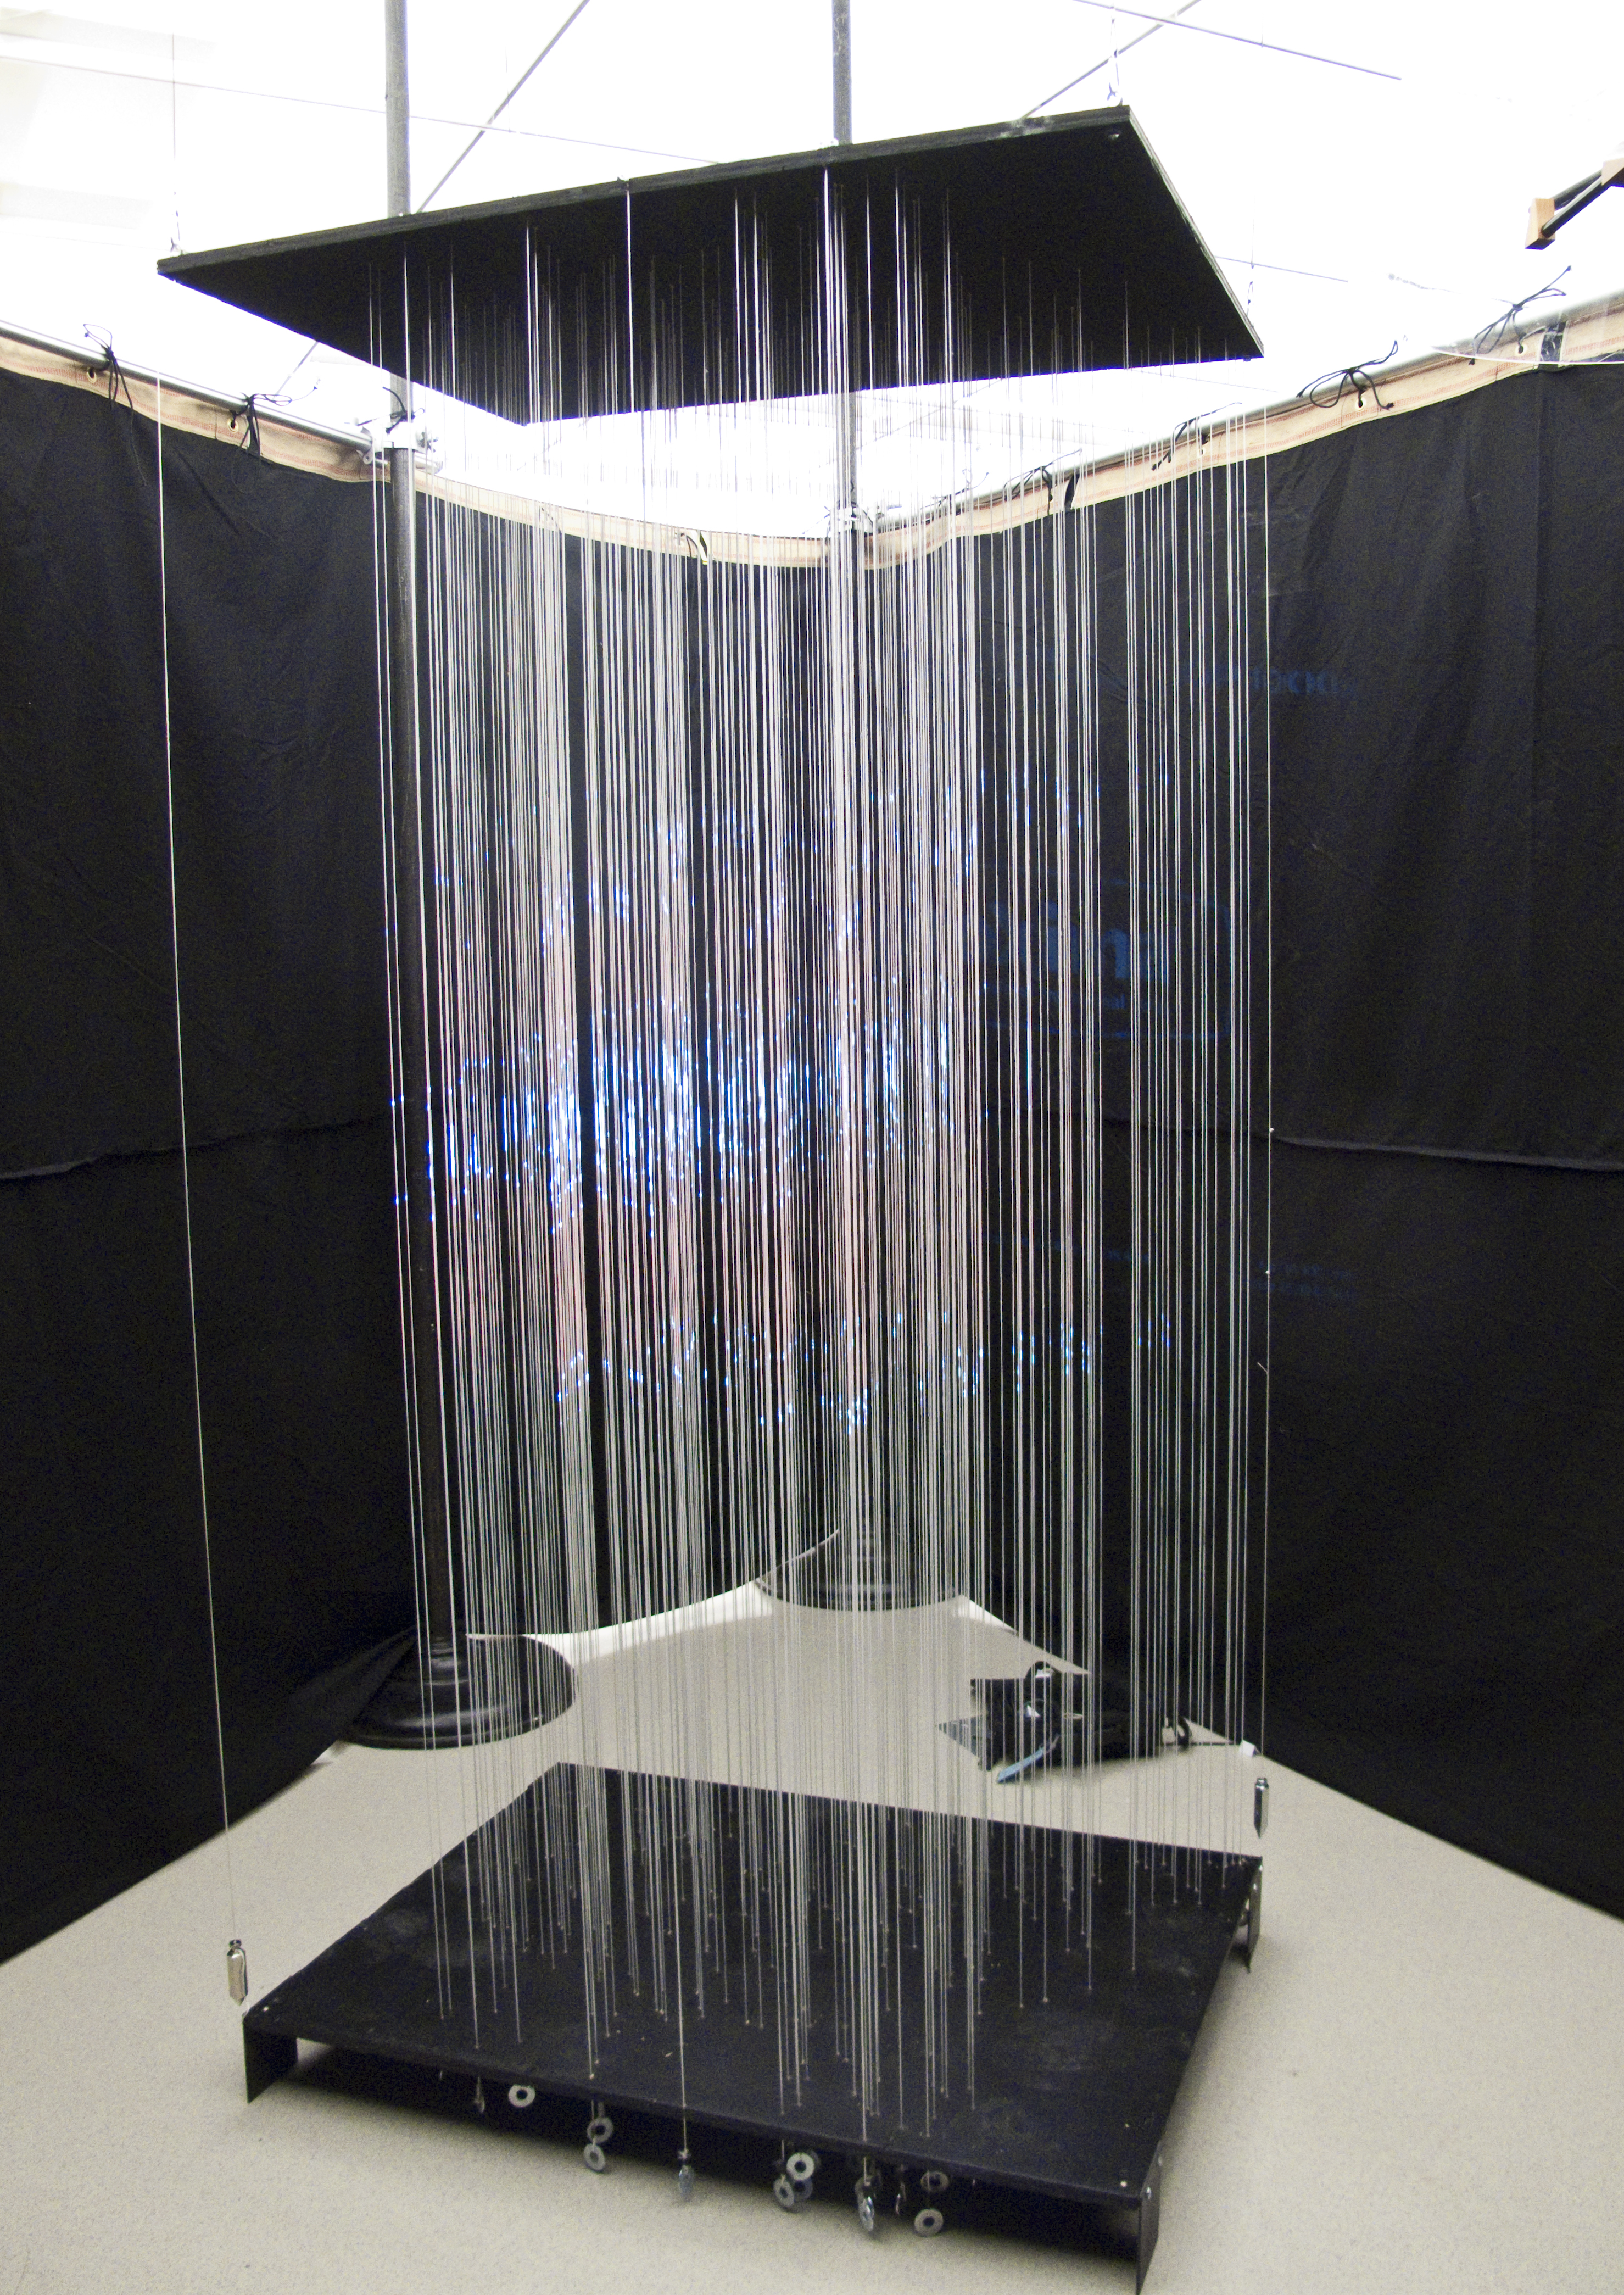
\includegraphics[width=.4\textwidth]{images/wiremapconst6.jpg}
  \caption{This is a Wiremap!}\label{fig:wmdiagram}
\end{figure}
\subsection{Wiremap Software Library}
In order to facilitate quicker prototyping and make the Wiremap software more accessible to the team, we wrote a simple Processing library for rendering certain shapes in the Wiremap field. The library replaces the source code provided by the creator of the Wiremap \cite{AH} by reducing code duplication and abstracting most of the implementation details away from a user who wishes to simply draw a sphere, rectangle or sliver in the field.

\paragraph{Abstraction}
The Wiremap library gathers the coordinate conversion and wire selection math into a single class. The previous method required duplicating a set of functions in every Processing sketch that output to the Wiremap. Now, the user creates an instance of the Wiremap class and provides a few key measurements of the physical interface as well as a text file listing the wire depths. The calculation is done as necessary, and not exposed to the user.

\paragraph{Coordinate Systems}
One key difference between the original source and the Wiremap library is the coordinate system used for each plane. Previously, the coordinates of X, Y and Z were all physical inches and matched the actual dimensions of the Wiremap. To facilitate quicker transitioning from a regular Processing sketch (using the standard 2D renderer) to one for the Wiremap, the X and Y were changed to be in the standard, Processing-style pixel coordinate system.

The Z plane remains in inches, as thre is no obvious relationship between Z space on the screen (which is infinite in both directions) and Z space in the Wiremap field (limited by the physical dimensions). Thus, Z coordinates in the field range from 0 to the field depth.

\paragraph{}The library has been released under the Apache open source license, and will continue to evolve after this project's completion. See the library's documentation for details on installation and usage \cite{CP}.
